\documentclass[
	12pt, % Default font size, values between 10pt-12pt are allowed
	%letterpaper, % Uncomment for US letter paper size
	%spanish, % Uncomment for Spanish
]{fphw}

% Template-specific packages
\usepackage{color} %red, green, blue, yellow, cyan, magenta, black, white
\usepackage[utf8]{inputenc} % Required for inputting international characters
\usepackage[T1]{fontenc} % Output font encoding for international characters
\usepackage{mathpazo} % Use the Palatino font
\usepackage{graphicx} % Required for including images
\usepackage{subfig}
\graphicspath{{figures/}}
\usepackage{array}
\usepackage{amsmath}
\usepackage{amssymb}
\usepackage{booktabs} % Required for better horizontal rules in tables
\usepackage{listings} % Required for insertion of code
\usepackage{enumerate} % To modify the enumerate environment
\usepackage[section]{placeins}
\usepackage{wrapfig}
\usepackage{pdfpages}
\usepackage[section]{placeins}
\usepackage{flafter}
%trying to do referencing using Chicago style
%NEW SHIT HERE
\usepackage{appendix}
%delete after, this is to place dummy text on the page
\usepackage[english]{babel}
\usepackage{setspace}
\usepackage{csquotes}
%how to use this package. Do your code snippets last, as you need to move the .m file into
%the same directory as this tex file

%adding a box around my imported latex code
\definecolor{mygreen}{RGB}{28,172,0} % color values Red, Green, Blue
\definecolor{mylilas}{RGB}{170,55,241}\lstset{frame=single, rulesepcolor=\color{black}, numbers=left}

\lstset{language=Matlab,%
    %basicstyle=\color{red},
    breaklines=true,%
    morekeywords={matlab2tikz},
    keywordstyle=\color{blue},%
    morekeywords=[2]{1}, keywordstyle=[2]{\color{black}},
    identifierstyle=\color{black},%
    stringstyle=\color{mylilas},
    commentstyle=\color{mygreen},%
    showstringspaces=false,%without this there will be a symbol in the places where there is a space
    numbers=left,%
    numberstyle={\tiny \color{black}},% size of the numbers
    numbersep=9pt, % this defines how far the numbers are from the text
    emph=[1]{for,end,break},emphstyle=[1]\color{red}, %some words to emphasise
    emph=[2]{word1,word2}, emphstyle=[2]{style},
}

\usepackage[authordate]{biblatex-chicago}
\DeclareFieldFormat[article]{title}{\mkbibquote{#1}} % make article titles in quotes
\DeclareFieldFormat[thesis]{title}{\mkbibemph{#1}} % make theses italics
\bibliography{Programming languages report}

\counterwithin*{equation}{section}
\counterwithin*{equation}{subsection}
\counterwithin*{equation}{subsubsection}

%CHANGE
%I want to save space when I am writing my document, so I am going to have
%everything as the default values for the system
%\setlength{\parindent}{0pt}
\setlength{\parskip}{1.0em}
%\onehalfspacing
%\setstretch{1.25}
%making a variable for where all my results are going to be stored
\newcommand\pathFiles{"summary/"}
%----------------------------------------------------------------------------------------
%	ASSIGNMENT INFORMATION
%----------------------------------------------------------------------------------------

\title{Programming Languages Assignment} % Assignment title
\author{Tawana Kwaramba: 19476700} % Student name
\date{October 25th, 2021} % Due date
\institute{Curtin University \\ Faculty of Science and Engineering: School of Electrical Engineering, computing and Math Science} % Institute or school name
\class{Programming Languages - COMP2007} % Course or class name
\professor{Ascsociate Lecturer: Arlen Brower}
%----------------------------------------------------------------------------------------

\begin{document}
\pagenumbering{gobble}
\maketitle
\newpage
\tableofcontents
\newpage
\listoffigures
%\newpage
\listoftables
\newpage
%\end{spacing}
\pagenumbering{arabic}
%----------------------------------------------------------------------------------------
%	Programming Languages Report
%----------------------------------------------------------------------------------------
\section{Introduction}

\section{Programme Testing and Programme execution}
Each programme folder in this assignment is going to have its own independent
\textbf{README.md}, and a \textbf{run.sh} file. Therefore, all the marker has to
do is to execute the run.sh file by typing \emph{./run.sh} and that will demonstrate
the functionality of my programme. It should be noted that practical
four doesn't contain a run.sh file instructions outlining on how the scripts
should be executed has being left in README.md.

\section{FORTRAN}
\subsection{Fortran: Discussion}
Fortran was based on the programming paradigm of the punch card system which imposed specific
rules on Fortran. Which included the following: the first column of each row is going to be reserved for
the comment character which is either a c or an asterisk ("c" or "*"); column one to five of each row
is going to be reserved for statements or labels; column six is going to be
reserved for the continuation of a command from the previous line; commands will
terminate on column seventy-two; and column seventy-three
to eighty are going to be reserved for sequence numbers. As a consequence, this
made Fortran more intellectually involving compared to previously written
languages of Java, C and Python. \par

Programming in Fortran I had to be more conscious on the current column number
which is typically not a behaviour I do while programming in the named languages.
In the named languages I would typically choose to keep each line below 80 characters
to make it easier for others to read the my code. Therefore, due to this imposed
rule Fortran's \emph{writability} is not like the named languages. \par

Fortran's variables is only limited to one-to-six characters long limiting the
expressivity of variables in Fortran. In some cases six characters is not enough
to fully explain the purpose of variable hence, compromises in variable naming
will have to be made. Compared to Java, C and Python the programmer can fully
express the purpose of variable as they is not limitation in variable name
length. Therefore, as demonstrated Fortran is less expressive in variable naming
as compared to Java, C and Python. Additionally, due to the limitation of the
variable length Fortran as well is going to break the \emph{zero-one-infinity}
programming principle. \par

Fortran doesn't support reserved words causing the change of behaviour of functions,
and resulting in a less \emph{reliable} programming experience. Programming in
Fortran requires double checking variable names to ensure that they were not
overriding in-built functions as the complier will not raise these incidents as
errors. As compared to the named languages the complier will raise the incidents
as errors, and the programmer typically would not have to concern themselves
with the naming of variables. Therefore, due to this Fortran will require the
programmer to involve themselves with behaviours which they're not accustomed too.
Additionally, since Fortran will allow the re-definition of in-build functions
meaning that in a programming project an intern can override a in-built function
to do something else and they would not know as the complier will not flag it i.e.
the do-while loop can be over ride to add one instead of looping. Hence, for this
reason programming in Fortran in less \emph{reliable} as compared to the named
languages.\par

Additionally, Fortran is less \emph{reliable} than Java, C and Python due the compilation
process. Fortran doesn't look for uninitialised variables hence, Fortran will
allow you to compile and run a programme even if the variable hasn't be declared
and not assigned to anything. Additionally, during execution the uninitialised
variable will be a random memory address thus, any operations in the programme
will be done to that specific memory address which in some cases can lead into
unintended actions resulting, in Fortran breaking the \emph{security} and
\emph{defense in depth} programming principle. As compared to the named languages
the complier will raise this incident as an \emph{uninitialised variable error}
therefore, stopping the user from accessing memory which they should not be accessing.
Therefore, as demonstrated Fortran in less \emph{reliable} and less \emph{secure}
than the names languages.\par

Similarities of Fortran as compared to the named programming languages is that
the first character of each variable has to start with a letter and can't start
with a number, Fortran will require you to declare the types of your variables
same as C, and Java. Furthermore, Fortran will require the programme fields to be
the same name as the current file name which is a similar idea which is seen in
java whereby the file name has to be the same as the class name, and Fortran will
require terminating statements for each command same as Java, and C.

\subsection{Fortran: reflection}
Fortran doesn't have scope as consequence it's difficult to plan and write
a full programme. As a result of no scope variables can be accessed from anywhere
causing unattended side effects as they is not protection from scope. Therefore,
this is going to make it harder to debug larger programmes, as the
programmer would have to have full knowledge of the programme instead
of knowledge of the current scope. Making Fortran difficult to structure code
in the appropriate hierarchies hence, violating the \emph{structured programming principle}.
Additionally, Fortran not allowing the hiding the implementation of abstract data
structures, and implementations violating the \emph{information hiding
principle}.\par


I found Fortran a lot harder to debug as the complier doesn't display helpful
messages. During this programming assignment I spent hours trying to figure
out why my programme was not working, although the logical structure of the
programme was correct. To only find out what it was due to that I had not
initialised a variable properly. Therefore, Fortran is not a language I would
personally use for large scale projects as the complier is not helpful. Additionally,
due to one small mistake breaking a programme Fortran is not \emph{reliable}.\par


Additionally, the complier will see all commands and variables as upper cases hence, making the language
case insensitive further adding on onto the \emph{unreliability} of the Fortran
programming language, as how would the programme know that they're going to be
accessing the correct variable or constant in the programme.\par
\section{ALGOL 68}
\subsection{ALGOL 68: Fizz-buzz Activation Record}
The programmed fizz buzz algorithm doesn't make use of actual functions, although
it makes use of in-built functions such as the print statement, and the read
statement. Therefore, the display can be illustrated as shown in figure \ref{ALGOL:Display},
and the accompanying static and dynamic chaining is demonstrated in figure \ref{ALGOL:Chaining}.
The construction of the display is based on the submitted ALGOL 68 implementation
of fizz-buzz.
\begin{figure}[!htb]
  \centering
  \begin{minipage}[b]{0.45\textwidth}
    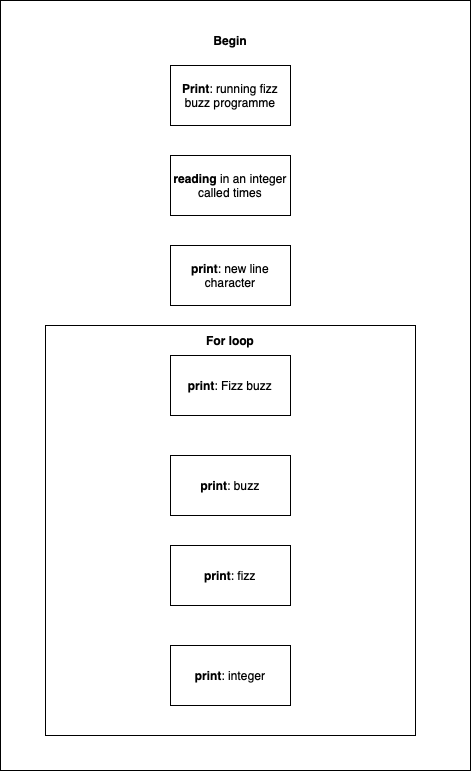
\includegraphics[width=\textwidth]{figures/algoDisplay.png}
    \caption{The display of the Fizz Buzz algorithm}
    \label{ALGOL:Display}
  \end{minipage}
  \hfill
  \begin{minipage}[b]{0.45\textwidth}
    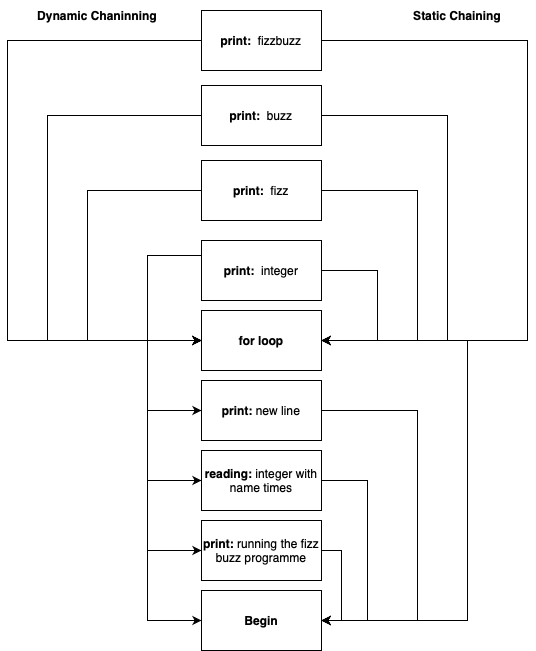
\includegraphics[width=\textwidth]{figures/stack.png}
    \caption{Static and dynamic chaining of the Fizz Buzz programme}
    \label{ALGOL:Chaining}
    \end{minipage}
\end{figure}

\subsection{ALGOL 68: reflection}
Writing the fizz buzz programme with ALGOL 68 was more pleasant than FORTRAN as
ALGOL 68 has started to represent languages which I am more accustomed too. \par

ALGOL 68 strongly reminds me of the bash scripting language as the constructs are going
to end with a word instead of terminating delimiter Therefore, looking at ALGOL 68
code is a lot easier, as all the constructs are clearly structured resulting in
compliance with the \emph{structured programming principle}. Additionally, since
the language is highly structured it's gong to be easier to read hence, complying
with the \emph{readability principle}. To me it almost seems like modern day
programming language structure was derived from ALGOL 68.\par

ALGOL 68 is going to be a language which is going to be scoped hence, the
variables which are in a \emph{begin} and \emph{end} block are only going to be
found to be accessed within that block, and variables which are going to be defined
in any given construct are going to be only accessed within those constructs.
Therefore in ALGOL 68 you're not going to get the side effects which you may get in
FORTRAN as the variables are going to be protected by scope resulting in ALGOL 68
adhering to the \emph{information hiding principle}. \par

\section{ADA}
\subsection{ADA: Comparison With C Bubble sort}
A difference between C and ADA Bubble sort is in the manner which they treat functions.
In C the construction of function which will return nothing or something
is going to have the same declaration, ADA separates the declaration of functions
which are going to return something and nothing. With functions returning nothing
being declared with the \emph{procedure} key word, and functions which are going to be
returning something declared as \emph{sub-routines}. Therefore, in the bubble
sort implementation, the swap, bubble-sort and display functions are going to be
declared as functions in C, and as procedures in ADA.\par

Another difference between C and ADA is going to be the choice of terminating characters
for commands. In C the end of a construct such as an if-and-else statement will
need to be terminated withe a semi-colon, and in C the end of a if-and-else
statement is going to be terminated with a right parenthesis. Therefore,
in the bubble sort algorithm where it checks if the leading number is going to be
less than the trailing number, ADA's if statement will terminate with a semi-colon,
and C will terminate with a parenthesis.\par

A similarity between C and ADA implementation is going to be found in the
positioning and definition of functions. In C this phenomenon is going to be
referred to as forward declaration whereby, the function header has to
be declared before the main body of code, in ADA the header and the function has
to be declared and implemented before the main body of code otherwise, ADA and C
complier will fail the programme. Therefore the swap, bubble-sort, and display
methods have to be declared in C's implementation of the bubble sort, and in ADA
the function has to be declared and implemented before the main method.
Furthermore, this idea will also extend to variable deceleration positioning, in C-89
implementations of bubble sort, as variables will have to be declared  before
any commands are, and in ADA variables and types will have to be declared before
the actual main body code, respective procedure and sub-routine functions.\par

Another similarity between the ADA and C implementation of bubble-sort is going
to be the use of pointer manipulation in order to swap any element which is
going to be greater than the element which is going to be in-front of the current
element. In both algorithms the elements to be sorted array is going to be
dereferenced, and then put swapped into the required position as seeing by the
swap function.\par


Furthermore, C and ADA are going to be both strongly type languages meaning,
that a variable or a data structure must be declared with a type before they're
going to be used. Therefore in the bubble sort implementation all variable names,
imports, and exports are going to require a type.

\subsection{ADA: reflection}
ADA has a unique manner of declaring it's variables which I think is a little bit
more readable as it follows the natural manner which we speak in. In ADA the variable
name will be declared first proceeded by the variable type, in other languages
such as Java an C the variable type will be declared first, and then the variable
name will be declared second. In the human language it's more logical to say
"A F-22 raptor is a plane", and not "a plane is a F-22 raptor" in this sentence
clearly the type is going to be a plane, and the name is F-22 raptor. The logical
most logical of constructing a sentence is to say the name followed by the type as
demonstrated in the example above which, is in the manner which ADA declares its
variables. Therefore, due to the manner of ADA's variable declaration  it will
make the language more readable.

\section{Yacc and Lex}
The first step in implementing symbol table is to choose the appropriate data
structure to store the symbols based on requirements. Given that compliers are
instruments which are used multiple times, and are going to be called multiply times
it's important that the chosen data structure will have a fast access time, an
ideal access time will be $$O(1)$$, and a more appropriate access time will be
$$O(nlogn)$$. Therefore, the more appropriate data structures to be chosen
will a form of a binary search tree, and or a hash table.\par

After chosen the appropriate data structure, the next thing to be decide is in
the manner which you're going to be accessing and setting your data in your data
structure, and how it's going to interface with the YACC file.\par

Then after, the symbol table can be implemented. Lex is going to server as the
tokeniser hence, it's going to declare what each part of a programme is going to
be, and Yacc is going to be where you grammar is going to be constructed hence,
it's going to given meaning to a programme. The combination of Yacc and Lex will
allow to create a parse tree. A parse tree is going to be a tree which is going
to represent the hierarchical syntactical structure of your programme which is
all the instructions ran in your programme and the root is going to be the actual
programme, and the branches are going to be the individual instructions in the
programme. Therefore, this parse tree is going to form your symbol table where as it
has all the variable and the accompanying type. Lastly, the parse tree has to
be stored in memory through the chosen data structure
in step one.

\subsection{reflection}
I really enjoyed the Yacc and Lex practical, although it was very time consuming
and painful to do. Overall, it was a good experience to see how the basis of
a programming complier is going to be constructed. Furthermore, doing this
practical gave on appreciation of some of the fundamental concepts taught in early
computing units. \par

A point of frustration while writing the programme is that the \emph{yytext}
variable was going to be a type of yystype which is going to be Yacc's own datatype
for defining a string. Therefore, during compilation I didn't think much about the
yystype warning, and as soon as I ran the programme through Yacc it produced segmentation faults.
Since, I thought the variable type yystype was just a warning, I thought it was going to be harmless.
This cardinal error lead into many hours of debugging, and playing around in Valgrind.
I would have wished the Yacc complier would have treated the data type mismatch
as an actually error as other languages such as java would have. Therefore,
since the complier will allow access of invalid memory addresses without any
other precautions Yacc will violate the \emph{defense in depth} principle. \par

Yacc and Lex code are both going to be segmented into sections, whereby the
first section is going to be the imports for the programme, then
it's going to be the definitions, the next section in the lex
file is going to be the tokenising rules and the corresponding return types,
in Yacc the next section is going to be the grammar of the
language, and finally the last section is going to be the C functions which are
going to be associated with each file. Due to the structured nature of the
programming language it made it easier to find area of interest i.e. if you want
to change the manner which Lex tokenize strings you can jump to the middle of the
file. Therefore, for this reason Yacc and Lex are going to adhere to the
\emph{structured programming principle} and as a consequence making the language
more \emph{readable}.\par

A good thing with Yacc is that it was really easy to pick up as it was heavily
coupled to the c language. Therefore, they was not that much to learn in the
Yacc language except on how it would process its language grammars.

\section{scripting languages}

\subsection{Scripting languages: discussion}
Although, I have used bash since starting my computer science
degree, and I use it in my daily navigation of the terminal environment I have
always find it hard to write in bash script. The reason why I think that bash
scripting is hardest to write is because it doesn't follow the common conventions
which I am accustomed to with C, Java, and Python. For example, if you want
to access a variable, it's not just enough to use its name like how you would
in Java, C and Python. You would have to access the variable name with a
\$ then you can use the desired variable.Furthermore,
if you want to declare a variable as something you will have to be cautious of your
spacing as in bash you can't have spaces before or after the assignment of your variable,
in languages such as Java, C, and Python they don't really care on how much spaces you
will have. These just some of bash conventions which are different from the
languages which I am accustomed too. Therefore, scripting is more difficult than
writing a programme in Java, C, and Python. Additionally, for this reason the
bash scripting was the hardest to write the find config file as they're going to
be a lot closer to modern day languages as discussed in the reflection.

\subsection{scripting languages: reflection}

\subsection{Bash} In conjunction to the points discussed above, bash will have different methods to
be able to access specific commands.The first method is going to be through the
name of the command, and the second method is going to be through the use of
the back-tick(`). These methods can't be sued inter-changeably some commands will
only work with the back tick method, and some of them with the name method hence,
adding another layer of complexity  while scripting. Therefore, the question then
becomes "am I accessing this command the right way", which is
typically not a question i would ask myself while writing other languages.
Therefore, in this regards bash will lack \emph{regularity}, and will add another
layer of difficulty while writing the language.\par


\subsubsection{Ruby} out of the three scripting languages done, ruby was the
easiest one to write in because it's a close representation to the python scripting
language, and java-script to some extent. Therefore, given that I have had a
vast experience in python in relation to industry projects, teaching, and
university assignment the \emph{wrtiability} of ruby was far better than bash,
and Perl.\par

Additionally, due to the close representation of ruby to other popular scripting
languages this makes ruby very easy to learn, and to understand what is being
conveyed in code. Furthermore, the syntax of ruby is very simplistic, and the
structure of the language closely represents what the programme's aim.
Therefore, in this manner ruby also adheres to the \emph{simplicity}
programming principle.

\subsubsection{Perl} in relation to the three scripting languages I would place
Perl as a middle child in relation to \emph{writiability}. Perl borrows syntactic
constructs, and conventions from both the bash scripting language, and modern
popular scripting languages such as python and java script. For example Perl
relays heavily on anonymous functions and calling functions within a function
as demonstrated in figure \ref{perl:demo} which is a design
pattern which is heavily used in java-script, and a little bit in Java. Additionally,
Perl only had fewer deviations from the conventional structure of modern day programming languages
for example with Perl, it doesn't really matter on how many blanks you have after
an assignment which follows normal programming conventions. Although, like bash
if you want to access a variable, the variable has to be proceeded with a dollar-sign
("\$"). Therefore, Perl borrows ideas from modern languages which I am accustomed too
and borrow ideas from Unix based scripting languages therefore, placing Perl as
a middle child in relation to \emph{writability}.

\begin{figure}[!htp]
    \begin{problem}
        \begin{verbatim}

        #files wanted is a reference to the address of a function

        find(\&filesWanted, $searchPath)
        sub filesWanted{

                #code for your function

            }
        \end{verbatim}
    \end{problem}
    \caption{Demonstration of Perl's design strucutre}
    \label{Perl:demo}
\end{figure}

\section{Small-talk}

\subsection{Small-talk: Discussion}

\subsection{Small-talk: Reflection}

Constructing the conditional statements was the hardest part of the small talk
practical this is because small talk doesn't natively have if-else-if statements,
and only has if-else statemnets. To simulate the if-else-if statement nature of the
programme, Small-talk will require you to nest an if-else staement inside the else
clause of the parent if-else statement as demonsstraed in figure \ref{ST:IF_ELSE}.For,
this reason it made writing the Small-talk programme more diffucult as I had to
keep a consicious note on the location and the number of terminating square brackers
("]") hence, in this regards Small-talk will have low \emph{writability}. Additionally,
for this reason, it's diffucult to see the purpose of the if-else structure from firs
glance as compared to the native if-else-if statements found in C, Java and Python. To
be able to understand the structure it would required the programme to actually
carefully read the programme and in this regards Small-talk is going to have
low \emph{readability}.

\begin{figure}[!htp]
    \begin{problem}
        \begin{verbatim}
        <True condition> ifTrue: [ <statment ] ifFalse:
        [ <child if-else-statement> ]
        \end{verbatim}
    \end{problem}
    \caption{Small talk if-else-if statments}
    \label{ST:IF_ELSE}
\end{figure}

\section{C++}

\subsection{C++:Discussion}

\subsection{C++: Reflection}
Out of the covered languages in the Programmning languages assignment, this was
probably the most intutive, easiest, and most well rounded programming languages as
compared to the ones coverred in the unit. This is due to that C++ is very similar
to programming languges which I have experience namely Java and C. Therefore,
writing the C++ programme was a lot easier as it follows most of the programing
principles which I am accoustmed too. C++ is \emph{reliable} as the complier is
very helpful in it's error messages and wil tell you exactly what is wrong in
your code. Additionally, the C++ is almost the same as Java and C syntax hence,
it was easier for me read the C++ programmes and to know the funcion of a
porgramme therefore, in this regards C++ is \emph{syntacically} consistent with
other languages; C++ is \emph{regular} as all groups of conditions and constructs
are going to be the same throughout the language; and C++ has the same structure
as Java, and C therefore it's \emph{structually} consistent with those languages
and also the strucutre of the language represents it's function and purpose therefor
adhering to the \emph{structured programming} principle.\par

C++ is a language which encourages the use of streams, and most of its constructs
is written to be used in conjuction with streams. However, C++ doesn't enforce
the use of streams as it iwll allow you to do operations in the manner which you're
accoustemed too hence, making the barrier in learning C++ a lot smaller, as other
languages will force you in doing thing their way. Therefore, for that reason
C++ is a lot easier to learn and to pick up if you have prior exprience to Java,
and C.

\section{Prolog}

\subsection{Prolog: Discussion}
Throughout my experience of programming I have only dealt with imperative languages
hence, languages which you tell what is should do at each every single step.
Prolog is a logical language whereby it's paradigm is that the programmer is
going to specify the world's rules and the world's facts, and the language is
going to make conclusions based on those rules and facts. Prolog is going to be
based on the idea of a decision tree where it will use forward chaining and
backwards chaining to form conclusions. For this reason writing the Prologa


\subsection{Prolog: Reflection}

\section{Scheme}

\subsection{Scheme: Discussion}

\subsection{Scheme: Reflection}





\end{document}
